% !TEX encoding = UTF-8 Unicode
\documentclass[a4paper]{article}

\usepackage{color}
\usepackage{url}
\usepackage[T2A]{fontenc} % enable Cyrillic fonts
\usepackage[utf8]{inputenc} % make weird characters work
\usepackage{graphicx}

\usepackage[english,serbian]{babel}
%\usepackage[english,serbianc]{babel} %ukljuciti babel sa ovim opcijama, umesto gornjim, ukoliko se koristi cirilica

\usepackage[unicode]{hyperref}
\hypersetup{colorlinks,citecolor=green,filecolor=green,linkcolor=blue,urlcolor=blue}

\usepackage{listings}

%\newtheorem{primer}{Пример}[section] %ćirilični primer
\newtheorem{primer}{Primer}[section]

\definecolor{mygreen}{rgb}{0,0.6,0}
\definecolor{mygray}{rgb}{0.5,0.5,0.5}
\definecolor{mymauve}{rgb}{0.58,0,0.82}

\lstset{ 
  backgroundcolor=\color{white},   % choose the background color; you must add \usepackage{color} or \usepackage{xcolor}; should come as last argument
  basicstyle=\scriptsize\ttfamily,        % the size of the fonts that are used for the code
  breakatwhitespace=false,         % sets if automatic breaks should only happen at whitespace
  breaklines=true,                 % sets automatic line breaking
  captionpos=b,                    % sets the caption-position to bottom
  commentstyle=\color{mygreen},    % comment style
  deletekeywords={...},            % if you want to delete keywords from the given language
  escapeinside={\%*}{*)},          % if you want to add LaTeX within your code
  extendedchars=true,              % lets you use non-ASCII characters; for 8-bits encodings only, does not work with UTF-8
  firstnumber=1000,                % start line enumeration with line 1000
  frame=single,	                   % adds a frame around the code
  keepspaces=true,                 % keeps spaces in text, useful for keeping indentation of code (possibly needs columns=flexible)
  keywordstyle=\color{blue},       % keyword style
  language=Python,                 % the language of the code
  morekeywords={*,...},            % if you want to add more keywords to the set
  numbers=left,                    % where to put the line-numbers; possible values are (none, left, right)
  numbersep=5pt,                   % how far the line-numbers are from the code
  numberstyle=\tiny\color{mygray}, % the style that is used for the line-numbers
  rulecolor=\color{black},         % if not set, the frame-color may be changed on line-breaks within not-black text (e.g. comments (green here))
  showspaces=false,                % show spaces everywhere adding particular underscores; it overrides 'showstringspaces'
  showstringspaces=false,          % underline spaces within strings only
  showtabs=false,                  % show tabs within strings adding particular underscores
  stepnumber=2,                    % the step between two line-numbers. If it's 1, each line will be numbered
  stringstyle=\color{mymauve},     % string literal style
  tabsize=2,	                   % sets default tabsize to 2 spaces
  title=\lstname                   % show the filename of files included with \lstinputlisting; also try caption instead of title
}

%Page break after paragraph title 
\makeatletter
\renewcommand\paragraph{\@startsection{paragraph}{4}{\z@}%
   {-3.25ex\@plus -1ex \@minus -.2ex}%
   {1.5ex \@plus .2ex}%
   {\normalfont\normalsize\bfseries}}
\makeatother
\begin{document}
\sloppy


\title{Hakovanje - večita igra nadmudrivanja\\ \small{Seminarski rad u okviru kursa\\Metodologija stručnog i naučnog rada\\ Matematički fakultet}}

\author{Nikola Dimić, Đorđe Pantelić, Nikola Živković,\\Mladen Canović\\ dimic.nikola@gmail.com, pantelicdjole94@gmail.com,\\nmzivkovic@gmail.com, mladen.canovic@gmail.com}

%\date{9.~april 2015.}

\maketitle

\abstract{
Ovaj rad ima za cilj da upozna čitaoca sa konceptima obmane, hakovanja i zlonamernim softverom. Kroz tehničke detalje, primere i savete o bezbednosti, otvoriće diskusiju o značaju sigurnosti na internetu. Kroz izučavanje tehnika i tehnologija koje predstavljaju jednu od najvećih opasnosti današnjice, cilj je napraviti kritički osvrt na bezbednost softvera i skrenuti pažnju na odgovornost, koja je postavljena pred moderno društvo.
}

\setcounter{tocdepth}{2}
\tableofcontents

\newpage

\section{Uvod}
\label{sec:uvod}
U originalnom značenju reč haker (eng. \textit{hacker}) je predstavljala osobu koja je, na kreativan način, pokušavala da modifikuje sistem tako da on radi nešto inovativno. Hakerska kultura nastala je na univerzitetu MIT (eng. \textit{Massachusetts Institute of Technology}) tokom pedesetih godina prošlog veka. Za njih \textit{hack} nije predstavljao samo unapređenje funkcionalnosti uređaja, već i prikaz njihove virtuoznosti. Nazvati nekoga hakerom, bio je izraz poštovanja \cite{ethics}.

U ovom radu biće reči o pojmu hakovanja kao i konkretnim primerima kroz koje ćemo se bolje upoznati sa konceptima 
upada i obmane \ref{hakovanje}. U nastavku rada, biće reči o tipovima zlonamernog softvera uz detaljnu analizu i primere. Za kraj, obratićemo pažnju na načine zaštite od ovog tipa softvera \ref{sec:malware}.

\section{Hakovanje}
\label{hakovanje}

Hakovanje (eng.~{\em Hacking}) predstavlja iskorišćavanje nedostataka sistema, računara ili računarskih mreža. Najčešća meta jesu ljudi koji rade na tom sistemu i ova vrsta napada predstavlja društveno inženjerstvo (eng. \textit{social engineering}).

Pored zlonamernih napadača (eng. \textit{Black hat}), postoje hakeri koji uz dozvolu administratora upadaju u sisteme u cilju testiranja njihove sigurnosti. Oni predstavljaju etičke hakere (eng. \textit{White hat}). Hakeri iz sive zone (eng. \textit{Gray hat}), zarad dokazivanja svojih veština, vrše napade bez dozvole, ali ne u nameri da nanesu značajnu štetu. Pored njih postoje hakeri koji se zalažu za određenu ideju ili cilj (eng. \textit{Hacktivists}), čiji su najpoznatiji predstavnici grupa Anonimusi (eng. \textit{Anonymous}) \cite{hackers_hat}.
 
\subsection{Umetnost upada}
\label{sec:intrusion}

Sa razvojem informacionih tehnologija i računarstva rasla je i pretnja od njihove zloupotrebe. Za hakovanje su interesovanje prvobitno pokazale mlade osobe, koje su se time bavile zbog ličnog uzbuđenja \ref{mladi_hakeri} ili grupe profesionalaca koje bi koristile svoju ekspertizu zarad materijalne dobiti \ref{milionska_prevara_kazina}. Danas države ulažu ogromna sredstva kako u bezbednost, tako i u regrutovanje talentovanih pojedinaca u političke svrhe i napade na vojne ciljeve \ref{cyberwarfare} \cite{intrusion}.

\subsubsection{Milionska prevara kazina}
\label{milionska_prevara_kazina}

Ranih devedesetih godina, Aleks Mejfild je sa tri prijatelja prezentovao softversko rešenje na konferenciji u Las Vegasu. Nakon posete kockarnici, došli su na ideju hakovanja poker aparata. Poker aparati su imali određene hardverske propuste - postojala je mogućnost zamene originalnog čipa. Zarad testiranja svojih programerskih sposobnosti oni su hakovali aparat na drugačiji način.

Napadači su kupili stariji aparat, jer ranije bezbednosti nije poklanjana velika pažnja, kako bi analizirali njegov algoritam. Koristeći disasembler, koji su sami razvili, preveli su izvršni kôd u izvorni. Analizom ključnih sekcija pronašli su generator nasumičnih brojeva iz šezdesetih godina, koji je predstavljao listu od oko četiri milijarde uskladištenih brojeva kroz koju se iteriralo na svaki deseti deo sekunde.

Po izvlačenju pet karata izvlačilo se još pet, koje bi bile rezerve u slučaju da igrač želi da zameni neke od prvobitno izvučenih. Tih deset karata predstavlja deset uzastopnih brojeva iz generatora. Pametnim rasporedom brojeva u početnoj listi, aparat kontroliše koja je tačno verovatnoća da igrač pobedi. 

Napadači su uz pomoć štoperice i programa, koji su razvili, znali tačno kada će aparat izbaciti dobitnu kombinaciju. Program je na osnovu prvobitno izvučenih karata mogao da odredi trenutno stanje generatora.
Nakon što se njihovo rešenje pokazalo kao uspešno, kupili su moderniji aparat kako bi povećali broj mesta na kojima mogu primeniti svoj metod. Ovaj aparat je imao dva generatora nasumičnih brojeva. Umesto da se svaka izvučena karta određuje na osnovu zbira generatora, iz istog razloga kao u prethodnom slučaju, za sve karte iz jednog izvlačenja korišćena je konstantna vrednost iz drugog generatora. Problem je ovim sveden na problem kriptografije gde su vrednosti prvog generatora pomerene za određeni korak koji se u svakom izvlačenju menja.

Za dve godine oštetili su kazino za preko milion dolara. Vremenom su napadači postali sve manje oprezni što je dovelo do otkrivanja njihove prevare. U zamenu za informacije o bezbednosnim propustima nisu procesuirani \cite{intrusion}.

\subsubsection{Informatičko ratovanje}
\label{cyberwarfare}

Informatičko ratovanje (eng. \textit{Cyberwarfare}) predstavlja način na koji države, bez stavljanja ljudskih života u opasnost, ostvaruju svoje ciljeve.

\textit{Stuxnet} je zlonamerni program otkriven 2010. godine koji je naneo ogromnu štetu iranskim nuklearnim elektranama. Pretpostavlja se da je delo američkih i izraelskih bezbednosnih agencija. Dizajniran je za napad na programabilne logičke kontrolere koji omogućavaju automatizaciju elektromehaničkih procesa, kao što je kontrola centrifugalnih mašina koje odvajajaju nuklearni materijal.

Koristeći četiri \textit{zero-day}\footnote{Zero-day propusti predstavljaju ranjivosti sistema za koje zna samo napadač.} propusta u operativnom sistemu \textit{Microsoft Windows}, virus je bio u mogućnosti da sebe iskopira na sve računare u lokalnoj mreži potpuno neprimetno. Kada bi se našao na nekom od računara \textit{Stuxnet} je menjao kôd \textit{Step7} alata kompanije \textit{Siemens} za upravljanje kontrolerima i ubrzavao rad centrifugalnih mašina kako bi vremenom došlo do njihovog kvara. Korisnicima bi bili prikazani lažni podaci na osnovu kojih se ne bi moglo zaključiti da nešto nije u redu. \textit{Stuxnet} se sastoji od tri modula od kojih jedan izvodi glavni deo napada, drugi prebacuje virus na ostale računare, a treći sakriva sve zlonamerne procese i datoteke kako bi onemogućio otkrivanje. U sistem je ubačen preko zaraženog \textit{USB} uređaja.

Na samitu o računarskoj bezbednosti u Meksiko Sitiju 2015. godine laboratorija Kasperski (rus. \textit{Лаборатория Касперского}) je objavila otkriće postojanja \textit{Equation} grupe, koja je dobila ime zbog izuzetno sofisticiranog algoritma za šifrovanje koji je razvila. Izveštaji navode da grupa postoji od 2001. godine. Zbog veoma naprednih tehnika i visokog nivoa prikrivenosti, grupa se povezuje sa Nacionalnom bezbednosnom agencijom (eng. \textit{National Security Agency, NSA}) Sjedinjenih Američkih Država. Otkriveno je da su pre, ili u isto vreme, koristili iste \textit{zero-day} napade koji su korišćeni i u virusu \textit{Stuxnet}, te se pretpostavljalo da su oni bili odgovorni za razvoj ovog virusa. Laboratorija Kasperski je grupu opisala kao daleko najsofisticiraniju koja je ikada otkrivena.

Pored virusa \textit{Stuxnet} povezuju se i sa zlonamernim programom \textit{Flame} otkrivenim 2012. godine koji predstavlja najkompleksniji virus ikada napravljen \cite{flame}. Sastoji se od deset grupa modula koji su prikazani u tabeli \ref{table:1}.

\begin{table}[h!]
\centering
\begin{tabular}{||c  c||} 
 \hline
 \textbf{Ime grupe} & \textbf{Namena} \\ 
 Flame & Moduli zaduženi za upad u sistem \\ 
 Boost & Moduli zaduženi za prikupljanje informacija \\
 Flask & Tip modula za napad \\
 Jimmy & Tip modula za napad \\
 Munch & Moduli za instalaciju i dalje širenje \\
 Snack & Moduli za lokalno širenje virusa \\
 Spotter & Moduli zaduženi za skeniranje sistema \\
 Transport & Moduli zaduženi za umnožavanje \\
 Euphoria & Slanje podataka ka ciljnim serverima \\
 Headache & Parametri i ostale karakteristike napada \\ [1ex] 
 \hline
\end{tabular}
\caption{Moduli zlonamernog programa Flame i njihova moguća namena}
\label{table:1}
\end{table}

Ovaj virus se koristio za špijunažu u zemljama Bliskog istoka, pretežno Iranu. Program je mogao da se širi preko lokalnih mreža, kao i preko uređaja koji poseduju {\em Bluetooth}. Mogao je nezapaženo da snima zvuk i ekran, da registruje unos sa tastature i svu komunikaciju preko mreže. Informacije je slao serverima koji su korišćeni za upravljanje i čekao dalja uputstva od njih. Posedovao je i \textit{kill} komandu koja je brisala sve tragove postojanja virusa na računaru, a koja je poslata odmah pošto je virus prvi put otkriven. U izveštaju laboratorije Kasperski se navodi da je \textit{Equation} grupa ta koja je pomogla napadačima, dok je \textit{CrySyS Lab}\footnote{ Laboratorija za kriptografiju i bezbednost sistema, Univerzitet tehnologije i ekonomije u Budimpešti.} kao odgovorne za razvoj virusa \textit{Flame} označio bezbednosnu agenciju zemlje sa ,,značajnim budžetom i kapacitetima`` \cite{flame}.

\subsection{Umetnost obmane}
\label{deception}

Sa razvojem bezbednosnih tehnologija, postaje sve teže
iskoristiti tehničke nedostatke sistema.
Posledica toga je sve veće iskorišćavanje ljudskog
faktora, što je često veoma lako. Vrsta napada, koji se
svodi na prevaru žrtve da oda poverljive informacije ili
napravi izmene u sistemu na kojem radi, a koje nisu u
njenom interesu, naziva se društveno inženjerstvo
(eng.~{\em social engineering}) \cite{deception}.

Osobe koje koriste nedostatke u ljudskoj prirodi, zarad ostvarenja svog cilja, nazivaju se društveni inženjeri (eng.~{\em social engineers}). Napadi društvenih inženjera uspevaju kada ljudi nisu dovoljno upoznati sa dobrom praksom u bezbednosti. Uprkos tome što kompanija ili pojedinac, zarad svoje bezbednosti, kupi sve moguće alate i obuči svoje zaposlene o merama predostrožnosti, ona je i dalje ranjiva jer je ljudski faktor najslabija karika bezbednosnog sistema.

Društveni inženjeri umeju sa ljudima, šarmantni su i harizmatični - osobine koje omogućavaju pridobijanje poverenja žrtve. Iskusni društveni inženjer, koristeći svoje umeće obmane, je u stanju da izvuče željenu informaciju ili inicira određenu radnju žrtve. Strategije za napad, koje oni koriste, sačinjene su od više različitih pristupa. Navedeni su neki od njih \cite{deception}.

\paragraph{Elementi strategija društvenih inženjera}
\begin{itemize}
\item \textbf{Skrivena vrednost informacija}

Društveni inženjeri često koriste informacije o firmi, koje su naizgled neinteresantne, a mogu biti od velikog značaja za ostvarenje cilja. Poznavanje osnovnih pravila, načina ponašanja i izražavanja, procedura, često korišćenih termina i skraćenica unutar firme ili unutar određenog odeljenja firme, mogu biti presudan faktor napada \ref{hack_za_ginisa}.

\item \textbf{Zloupotreba poverenja}

Poverenje je ključ prevare. Društveni inženjeri 
planiraju svoj napad vrlo temeljno, pokušavajući da 
predvide pitanja koja bi žrtva mogla postaviti. Vode 
razgovor koji, za žrtvu, ne izlazi van okvira 
uobičajenog. Kada žrtve nemaju razloga za sumnju, 
napadačima je lako da pridobiju njihovo poverenje i, 
koristeći svoje veštine, ostvare svoje namere.

\item \textbf{Pomoć neprijatelja}

Kada su ljudi uplašeni ili pod određenim pritiskom 
zbog nekog problema, skloni su da prihvate savete od 
osoba, koje ostavljaju utisak poverenja, a koje nikada
nisu sreli. Napadač kroz pružanje pomoći žrtvi
ostvaruje svoje ciljeve. On navodi žrtvu da instalira 
zlonamerni softver ili otkrije poverljive informacije, koje žrtva prepušta u nadi da će dovesti do rešenja 
problema. Početni problem može biti prouzrokovan od strane napadača \ref{pomoc_neprijatelja}.

\item \textbf{Iskorišćavanje osećanja}

Iskusni društveni inženjeri su vešti u manipulisanju 
osećanjima žrtve. To čine koristeći psihološke okidače (eng.~{\em psychological 
triggers})\footnote{Automatski mehanizmi ljudske psihologije koji ih čine podložnim sugestiji.}, koji 
dovode do površnog pristupa žrtve problemu bez 
temeljne analize dostupnih informacija. Napadač 
izaziva saosećajnost žrtve izmišljajući problem, koji 
je žrtva prethodno i sama iskusila. Pored ovog 
pristupa, napadač može izazvati osećaj krivice kod 
žrtve ili koristiti zastrašivanje kao oružje.
\end{itemize}


\subsubsection{Najveća računarska prevara u istoriji}
\label{hack_za_ginisa}

Stenli Rifkin je, 1978. godine, radio za kompaniju 
zaduženu za razvoj sistema za bezbednost jedne od 
najvećih banaka u Los Anđelesu, pa je imao pristup 
poverljivim informacijama te banke. Radeći na 
odeljenju za prenos novca na daljinu (eng.~{\em wire 
room}), upoznao se sa procedurom transakcija. 
Službenici koji su imali ovlašćenje da nalože 
transfer, svakog jutra su dobijali kôd koji su u toku 
tog dana koristili u procesu autorizacije. Službenici 
bi najčešće napisali tu šifru na parčetu papira i 
ostavili je na sebi vidno mesto. 

Izvršavajući svoja zaduženja na odeljenju, uspeo je da pročita aktuelni kôd sa parčeta papira jednog od službenika i da ga zapamti. Otišao je do govornice, odakle je pozvao jednog od zaposlenih u odeljenju za prenos novca i predstavio se kao član međunarodnog odeljenja banke.
Posle uspešne autorizacije kôdom službenika, naložio je prenos deset miliona dolara na račun u Švajcarskoj, koji je prethodno otvorio. Postojao je deo koji je napadač propustio prilikom upoznavanja sa samom procedurom. Bio mu je potreban i broj međupartijskog poravnanja (eng.~{\em interoffice settlement number}). Nazvao je drugo odeljenje u banci, predstavio se kao zaposleni sa kojim je upravo razgovarao i tražio broj koji mu je nedostajao, uz obrazloženje da ga je zaboravio. Kada je saznao broj, ponovo je pozvao sobu za transfer novca na daljinu i uspešno završio transakciju. 

U Švajcarskoj je podigao novac kojim je kupio dijamante, koje je kasnije u kaišu prošvercovao nazad. Iako za ovaj poduhvat nije koristio računar, njegova prevara ušla je u Ginisovu knjigu rekorda u kategoriji ,,najveća računarska prevara`` \cite{deception}.

\subsubsection{Zloupotreba poverenja}
\label{pomoc_neprijatelja}

Napadač Bobi Volas je nazvao zaposlenog u kompaniji 
\textit{Starboard shipbuilding}, čije tajne podatke je želeo da sazna i predstavio se kao tehnička podrška. Obavestio ga je da su u narednom periodu mogući problemi na mreži i da u slučaju nekog kvara pozove prvo njega. Posle nekoliko dana je pozvao mrežni operativni centar kompanije i predstavio se kao zaposleni u kompaniji, koristeći podatke radnika, kojeg je prvobitno nazvao. Od operatera je tražio da isključe mrežu u njegovoj kancelariji, kako bi otklonio kvar. Sada je mreža, u kancelariji žrtve napada, bila isključena, pa nije mogao da preuzme potrebne datoteke sa servera, razmenjuje informacije sa kolegama, proveri elektronsku poštu ili koristi štampač.

Zaposleni je, upozoren da do ovoga može doći, pozvao broj koji je nekoliko dana pre toga dobio od napadača. Napadač se trudio da zvuči željno da pomogne kolegi u nevolji, ali i da ga ubedi da mu pružanjem te pomoći čini veliku uslugu. Nakon nekog vremena pozvao je mrežni operativni centar i zatražio uključenje mreže. Posle toga je ponovo pozvao zaposlenog i koristeći osećaj zahvalnosti koji je otklanjanjem problema izazvao, lako ga ubedio da instalira aplikaciju, koju mu je predstavio kao zaštitu od budućih problema sa mrežom. U pitanju je bio računarski virus - trojanski konj \ref{Odisej}, koji je napadaču omogućio potpunu kontrolu nad žrtvinim računarom \cite{deception}.

\subsubsection{Odgovornost modernog društva}

Meta napada može biti stanovništvo nekog područja ili zemlje. Ova aktivnost se naziva društveno inženjerstvo velikih razmera (eng. \textit{large scale social engineering}) i izvode je velike organizacije ili države u cilju pomeranja javnog mnjenja u željenom pravcu. Predstavlja sofisticiran oblik propagande\footnote{Širenje pristrasnih i neobjektivnih informacija zarad promocije određenih ideja.}. Najčešći način napada je korišćenje pametnih sistema ili dobro organizovanih pojedinaca za sinhronizovanu aktivnost na društvenim mrežama i širenje lažnih vesti (eng. \textit{fake news}) putem botova\footnote{Nalozi sa lažnim identitetima kojima upravlja neki pojedinac ili pametni sistem.} (eng. \textit{bot}). Osim napada na druge \ref{no_collusion_witch_hunt}, vlade ga koriste i za propagandno delovanje nad svojim stanovništvom. Pred modernim društvom nalazi se veliki izazov kako pravno regulisati ove pojave na društvenim mrežama koje utiču na demokratske procese, a na pojedincima je velika odgovornost da svemu pristupaju sa dozom kritičkog mišljenja i donose utemeljene zaključke \cite{fake_news}.


\section{Zlonamerni softver}
\label{sec:malware}

Zlonamerni softver (eng.~{\em Malware}) predstavlja softver koji je dizajniran tako da nanese štetu ciljnom korisniku. U zavisnosti od namene, funkcije i opasnosti, postoji više vrsta zlonamernog softvera. Manje opasni programi mogu samo zauzeti procesorsko vreme ili mesto u memoriji i na taj način usporiti rad računara, dok opasniji mogu uništiti podatke na računaru, pa čak i preuzeti potpunu kontrolu nad njim. Na taj način računar postaje alat koji se može upotrebljavati za razne ilegalne aktivnosti, poput krađe kreditnih kartica ili napada na druge računare u mreži \cite{ethics}.


\subsection{Virusi}

Računarski virus je program koji se ugrađuje u izvršni kôd drugih programa. Namena računarskog virusa je da zarazi sistem, koristeći loše obezbeđene delove, preuzme kontrolu ili ukrade poverljive podatke. Načini na koje se virus širi su otvaranje dodatka (eng.~{\em attachment}) u okviru elektronske pošte, poseta zaraženom sajtu, pokretanje neproverene izvršne datoteke ili povezivanje zaraženog prenosnog uređaja sa računarom. Računarski virus može raditi na dva načina. Može se aktivirati čim dospe u sistem ili naknadnom akcijom korisnika \cite{viruses_and_worms,computer_virus}.
\paragraph{Tipovi virusa}
\begin{itemize}
\item \textbf{Virus sektora za podizanje sistema}

Virus sektora za podizanje sistema (eng. \textit{boot sector virus}) napada uređaje za skladištenje podataka, kao što su tvrdi (eng. \textit{hard drive}) ili flopi (eng. \textit{floppy}) diskovi, tako što izmeni njihovu glavnu sekciju za podizanje sistema. Kada se sistem jednom podigne sa zaraženim programom, virus se učita u radnu memoriju i dalje širi na sve flopi diskove ubačene u računar. Kako se u moderne operativne sisteme ugrađuju čuvari te kritične sekcije (eng. \textit{safeguard}), a flopi diskovi su izašli iz upotrebe, ovaj tip virusa je prevaziđen \cite{viruses_and_worms, computer_virus}.


\item \textbf{Virus direktnih akcija}

Virus direktnih akcija (eng. \textit{direct action virus}) se aktivira čim dospe u sistem, ne sakriva se u memoriji i cilj mu je da se svakim izvršavanjem dodatno proširi kroz sistem. Virus inficira najpre tipove datoteka koje napadač odredi, a zatim i sistemske datoteke odgovorne za određene operacije prilikom podizanja sistema. Ovaj tip virusa nema za cilj brisanje datoteka ili smanjivanje performansi računara već prikupljanje i menjanje pristupa određenim podacima. Antivirusi veoma lako primete aktivnosti ovog tipa virusa \cite{directaction}.


\item \textbf{Prikriveni virus}

Nasuprot virusu direktnih akcija prikriveni virus (eng. \textit{resident virus}) je specifičan po tome da ga je teško identifikovati i odstraniti. Virus se instalira na sistem i krije u memoriji računara. Modularan je, pa je tako svaki deo virusa zadužen za različitu zlonamernu aktivnost. Korišćenje ovakvog tipa virusa indukovano je poznavanjem značajnih propusta na samom sistemu \cite{computer_virus}.

\item \textbf{Polimorfni virus}

Polimorfni virus (eng. \textit{polymorphic virus}) je imun na tradicionalne antivirus programe. Ovaj tip virusa menja svoj izvršni kôd svaki put kada se kopira. Ovo dovodi do otežanog lociranja virusa pomoću antivirus programa, kao i do toga da se sam virus brzo širi kroz ceo sistem \cite{computer_virus}.

\item \textbf{Prepisujući virus}

Prepisujući virus (eng. \textit{overwrite virus}) je jedan od najjednostavnijih virusa. Odlikuje se time što briše originalan kôd zaraženog programa i menja ga novim, zlonamernim kôdom. Kada se novonastali program pokrene, virus se širi kroz sistem. Kako zlonamerni program briše zaraženu datoteku parcijalno ili u celosti, nije moguće povratiti je \cite{overwriting_virus}.

\item \textbf{Virus koji koristi prazan prostor}

Virus koji koristi prazan prostor (eng. \textit{spacefiller}) popunjava prazna mesta na zaraženom disku ili u izvršnom kôdu zaraženih datoteka. Prostor popunjava sopstvenim kopijama pri čemu se veličina originalne datoteke ne menja, stoga ga je veoma teško primetiti \cite{spacefiller_virus}.

\end{itemize}


\subsection{Softver za špijuniranje}
\label{spyware}
Softver za špijuniranje (eng. \textit{Spyware}) je neželjeni softver koji upada u sistem i krade poverljive informacije. Ovaj softver sakuplja lične podatke korisnika i šalje ih zlonamernim pojedincima ili kompanijama, koje se bave reklamama ili obradom podataka. Cilj softvera je da dođe do lozinki i finansijski osetljivih podataka žrtve. Virus prati aktivnost korisnika na internetu i čuva njegove informacije pri prijavljivanju na veb stranice. Neki tipovi softvera za špijuniranje mogu da instaliraju dodatne neželjene programe na uređaj, kao i da menjaju podešavanja \cite{spyware}.

\paragraph{Tipovi softvera za špijuniranje}
\begin{itemize}
\item \textbf{Adver}

Adver (eng. \textit{Adware}) se koristi u svrhu marketinga, tako što prati istoriju pretraživanja i preuzete podatke sa interneta, sa namerom da predvidi kakvi bi proizvodi zainteresovali korisnika i te informacije prosleđuje marketinškim agencijama. Može znatno da uspori računar \cite{spyware}.

\item \textbf{Kolačići za praćenje}

Kolačići za praćenje (eng.~{\em tracking cookies}) prate sve akcije korisnika na internetu, kao što su istorija pretraživanja ili razmena podataka. Njihova podrazumevana namena nije zlonamerna, ali mogu da se iskoriste od strane sajber kriminalaca (eng. \textit{cyber criminal}) \cite{tracking_cookies}.

\item \textbf{Posmatrači sistema}

Posmatrači sistema (eng.~{\em system monitors}) prate sve akcije korisnika na računaru, registruju svaki pritisak dugmeta na tastaturi, pročitanu elektronsku poštu, razgovor na internetu, posećene veb stranice i korišćene programe \cite{spyware}.
    
\end{itemize}

\subsection{Trojanski konj}
\label{Odisej}

Trojanski konj (eng.~{\em Trojan horse}), nazvan po čuvenom Trojanskom konju iz Homerovog epa \textit{Odiseja}, predstavlja štetni program. Maskiran je u program koji je koristan, dok u pozadini izvršava zlonamerne akcije bez znanja korisnika \cite{trojanhorse}.

Primer trojanskog konja predstavlja softver \textit{Mocmex}, otkriven 2008. godine, koji se nalazio na digitalnim ramovima za slike u Kini. Umesto isključivog učitavanja slika ovaj softver je, kada bi bio priključen na računar, prikriveno krao lične informacije o korisnicima, šifre za \textit{MMORPG} (eng. \textit{Massively multiplayer online role-playing game}) i slično. \cite{ethics}. 

\subsection{Mreža botova}
\label{botnet}

Mreža botova (eng.~{\em Botnet}) je kolekcija 
međusobno povezanih zaraženih uređaja, koji su pod kontrolom istog tipa zlonamernog softvera. Korisnici zaraženih uređaja često nisu svesni da je njihov sistem deo mreže botova.

Zaraženi uređaji se kontrolišu daljinski, bez 
korišćenja značajnih resursa računara, tako da njihove zlonamerne akcije bivaju sakrivene od korisnika. Mreže botova se koriste za slanje neželjene elektronske 
pošte ili preusmeravanje korisnika na zlonamerne veb 
stranice. Mreža botova napada nedovoljno zaštićene 
uređaje, sa ciljem da se proširi na što više uređaja i da se računarska moć i resursi, kojima mreža 
raspolaže, iskoriste za automatske radnje koje ostaju 
skrivene od korisnika. Da bi ostala skrivena, mreža 
koristi neprimetno mali protok podataka. 

Mreža koja broji milione uređaja može da proizvede ogroman saobraćaj na željenim veb stranicama i na taj način, potpuno neprimećeno, napadačima donese materijalnu dobit. Može se koristiti i za \textit{DDoS} napade (eng. \textit{Distributed Denial of Service attack}). Ovi napadi otežavaju rad servera, tako što ga zatrpavaju velikom količinom zahteva \cite{botnet}.

\subsubsection{Arhitektura mreže botova}

Kada inficiraju željeni broj uređaja, napadači mogu da kontrolišu mrežu na dva različita načina. Tradicionalni klijent/server pristup uključuje postavljanje kontrolnog servera (eng.~{\em Command and Control server}), koji šalje automatske komande botovima koristeći komunikacione protokole, kao što je \textit{IRC} protokol (eng.~{\em Internet Relay Chat}). Botovi su u stanju čekanja, sve dok ne stigne naredba sa kontrolnog servera.

Drugi, decentralizovani pristup uključuje mrežu ravnopravnih korisnika (eng.~{\em peer-to-peer}). Zaraženi uređaji komuniciraju unutar mreže i tako dele nove naredbe najskorije verzije zlonamernog softvera, koji njima upravlja \cite{botnet}.

\subsection{Računarski crvi}
Računarski crv (eng.~{\em Computer worm}) je zlonamerni program koji se umnožava širenjem kroz mrežu međusobno povezanih računara. Širenje crva unutar mreže uslovljeno je propustima u toj mreži ili operativnom sistemu \cite{norton_worm, ethics}. Na slici \ref{fig:crvsirenje} prikazana je ilustracija širenja računarskog crva kroz mrežu.

\begin{figure}[h!]
\begin{center}
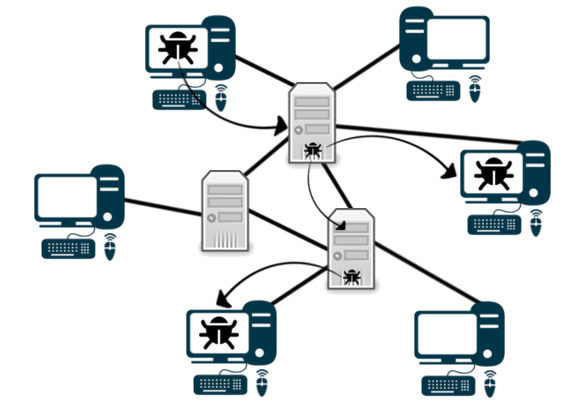
\includegraphics[scale=0.35]{worms.png}
\end{center}
\caption{Širenje računarskog crva kroz mrežu}
\label{fig:crvsirenje}
\end{figure}

Računarski crv ne mora nužno biti zlonameran, ali uvek vrši neku vrstu ugrožavanja sistema, makar kroz usporavanje protoka podataka kroz mrežu. Česta primena crva je da kroz veliko širenje omogući uslove za druge vrste napada \ref{botnet}. U tom slučaju, crv instalira program pomoću kojeg se tim računarom može daljinski upravljati \cite{ethics}.

Ideja o ovakvom tipu softvera prvi put je predstavljena u naučno-fantastičnom romanu napisanom 1975. godine, autora Džona Brunera, u kom se pominju crvi, programi koji se šire kroz mrežu futurističkih računara. Nedugo zatim, 1979. godine, nekolicina zaposlenih u firmi ~{\em PARC} u Kaliforniji pravi i testira ovakav tip programa.
Prvi računarski crv je zapravo bio dobronameran. Korišćen je za brzo širenje korisnih informacija kroz mrežu \cite{internet_worm}. 


\subsubsection{Internet crv}

Termin Internet crv  (eng.~{\em Internet worm}) se najčešće poistovećuje sa terminom Morisov crv, odnosno programom Roberta Morisa, koji je drugog novembra 1988. godine naneo višemilionsku štetu korisnicima interneta u Americi. Ovo je prvi napad korišćenjem ovakvog tipa programa i kao takav je dobio veliku pažnju medija i javnosti \cite{ethics}.

Internet crv je koristio greške u samom kôdu~{\em Unix} operativnog sistema, u komandama~{\em fingerd} i~{\em sendmail}, kao i tehnike za otkrivanje jednostavnih lozinki i brzo se proširio kroz mrežu na računare vojske, univerziteta pa i bolnica. Usled greške u samom kôdu crva, program se kopirao na iste računare po par stotina puta. Ovo je dovelo do toga da brojni računari otkažu usled prevelikog broja programa koji se na njima izvršavaju. \cite{internet_worm}.


\subsubsection{Saser}
Saser (eng.~{\em Sasser}) je vrsta računarskog programa, koji je izazvao velike troškove i podigao svest javnosti o važnosti ažuriranja softvera. Pušten je u opticaj 2004. godine. Saser je za širenje na skoro 18 miliona računara širom sveta iskoristio grešku u starijoj verziji~{\em Windows} operativnog sistema. Tako su računari koji nisu imali aktuelnu verziju operativnog sistema, među kojima su bili računari austrijske železnice i britanske obalske straže, postali neupotrebljivi \cite{ethics}.

\subsection{Ukrštanje veb lokacija}

Koristeći tehniku ukrštanja veb lokacija (eng.~{\em Cross-Site scripting}), zlonamerni korisnik može 
postaviti kôd unutar veb stranice, iskorišćavajući 
propuste u bezbednosti. Postavljen kôd se izvršava u 
trenutku kada korisnik poseti datu stranicu i tada 
napadač najčešće dolazi do informacija o njemu. \cite{ethics,xss}.

Primer propusta na veb stranicama je način čuvanja komentara na serveru. Komentari se čuvaju u bazi podataka bez obrade ili provere, a zatim prikazuju na klijentskoj strani veb aplikacije. Napadač, ostavljanjem komentara u određenom formatu, postavlja zlonamerni kôd. Kôd može izmeniti stranicu, tako da se prilikom posete korisnika veb aplikaciji aktivira program, koji šalje podatke korisnika napadaču. Ti podaci su uglavnom kolačići, ali mogu predstavljati lozinke i druge osetljive podatke \cite{xss}.

\subsection{Usputno preuzimanje podataka }

Usputno preuzimanje podataka (eng.~{\em Drive by downloads}) predstavlja napad na računar posetioca zaražene veb stranice, tako što se na njegov računar kopiraju zlonamerne datoteke. Napadač može izmeniti
loše obezbeđenu veb stranicu, tako da se na računar 
svakog posetioca te stranice kopira određeni 
zlonamerni program, bez znanja korisnika. Posetilac 
može postati žrtva napada i svesnim preuzimanjem 
softvera sa zaražene veb stranice, čija namena je 
različita od predstavljene \cite{drivebydownloads, ethics}.

\subsection{Mere zaštite od zlonamernog softvera}

Nemoguće je u potpunosti se odbraniti od napada, ali je moguće rizik svesti na minimum. Tri odbrambene mere, koje su najvažnije za očuvanje sistema navedene su u narednoj listi. 

\begin{itemize}
\item \textbf{Bezbednosne zakrpe softvera}

Bezbednosne zakrpe softvera (eng. \textit{Security patches}) predstavljaju ažurirane delove softverskog 
rešenja, koje je u svojim prethodnim verzijama sadržalo određene propuste, od kojih su neki otkriveni nakon pretrpljenih posledica.


\item \textbf{Alati za odbranu od zlonamernog softvera}

Alati za odbranu od zlonamernog softvera (eng. \textit{antimalware tools}) se koriste u preventivne svrhe ili za analizu i otklanjanje zaraženih datoteka, uz prethodnu saglasnost korisnika. Zbog naglog povećanja broja vrsta zlonamernog softvera i tehnika napada, potrebno je redovno ažurirati ove alate.

\item \textbf{Zaštitni zidovi}

Zaštitni zidovi (eng. \textit{firewalls}) predstavljaju softver koji se koristi za regulisanje mrežnog saobraćaja na računaru. Zaštitni zidovi omogućavaju korisniku da odabere koja će aplikacija imati pristup internetu. Ne pružaju dovoljnu zaštitu ukoliko su računari već zaraženi tipom zlonamernog softvera koji može onesposobiti zaštitni zid \cite{ethics}.

\end{itemize}

\section{Zaključak}
\label{sec:zakljucak}

Kroz ovaj rad se moglo ustanoviti da je obezbeđenje često iluzija sigurnosti \cite{deception}. Kroz osvrt na različite vrste napada i tehnika obmane se mogao steći utisak o manama bezbednosnih sistema. Unapređivanjem tih sistema unapređuju se i tehnike napada, pa njihov odnos predstavlja povratnu spregu bez konačnog pobednika. 
Prednost napadača je to što sigurnosni sistem mora da pobedi svaki put, dok je njemu dovoljno da pobedi samo jednom \cite{intrusion}.


\addcontentsline{toc}{section}{Literatura}
\appendix
\bibliography{seminarski} 
\bibliographystyle{plain}

\appendix
\section{Dodatak}

\subsection{Hakovanje zarad uzbuđenja}
\label{mladi_hakeri}

Džonatan Džejms, u potpisu \textit{Comrade}, je najmlađa osoba ikada osuđena za hakovanje na teritoriji Sjedinjenih Američkih Država. Njegov prijatelj \textit{Ne0h} je već sa deset godina počeo da se bavi hakovanjem.  \textit{Comrade} i 
\textit{Ne0h} su se upoznali preko sajtova koji su predstavljali sobe u kojima su ljudi sličnih interesovanja mogli da razmenjuju informacije u tekstualnom formatu (eng. \textit{Internet Relay Chat, IRC}). Hakeri se često udružuju u grupe kako bi razmenjivali informacije i organizovali grupne napade.

Sredinom 1998. godine na jednom od tih sajtova \textit{Comrade} je stupio u kontakt sa Halidom Ibrahimom, čovekom za koga se u zajednici pričalo da regrutuje ljude za upade na vladine sajtove i koji radi za, tada ne toliko poznatog teroristu, Bin Ladena. Halid je stupio u kontakt i sa \textit{Ne0h}-om kome je obećao 1000\$ ukoliko uspe da hakuje tehnički univerzitet u Kini. Ovaj zadatak, koji je bio samo test njegovih sposobnosti, je uspešno obavio.

Nakon nekoliko uspešnih probnih zadataka, od njega je zatraženo da hakuje avio kompaniju Boing (eng. \textit{Boeing}). \textit{Ne0h} je uspeo da provali širi obruč mreže i ostavi program koji mu je dao uvid u sve dolazne i odlazne pakete (eng. \textit{sniffer}). Na ovaj način uspeo je da sazna nekoliko korisničkih imena i lozinki koji su mu omogućili da uđe dublje u sistem. Uspeo je da dođe u posed i isporuči Halidu šeme vrata na avionu Boing 747, šemu pilotske kabine, kao i celog nosa aviona. Za \textit{Comrade}-a je imao  zadatak da hakuje \textit{SIPRNET}\footnote{Mreža koju je koristila vojska i druge vladine bezbednosne agencije za brz prenos naređenja na celoj teritoriji države.}. Iako je ovo predstavljalo ogroman rizik uspeo je da na nekoliko računara na mreži ostavi program koji je pratio komunikaciju.

U isto vreme, u Indiji su teroristi oteli avion. Sleteli su u Avganistan i tu čekali osam dana dok vlasti nisu pristale da oslobode trojicu ekstremista iz zatvora. Među njima bio je i Šîh Umer, koji će kasnije postati glavni finansijer Muhameda Ate, vođe terorista koji su izveli napad 9.11.2001. Halid je u razgovoru sa \textit{Comrade}-om rekao da je i on sam bio deo otmice. Nakon ovoga, počeo je da uklanja tragove svojih aktivnosti povezanih sa njim.

Nekoliko dana posle njegovog upada u \textit{SIPRNET}, njegovog oca je kontaktirao \textit{FBI}. Vlasnik računara na koji je uspeo da se infiltrira, bila je \textit{NASA} (eng. \textit{National Aeronautics and Space Administration}). Optužen je za tronedeljni 
zastoj u radu te organizacije, kao i za presretanje 
elektronske pošte ministarstva odbrane. Na jednom od 
njegovih diskova pronađen je program koji bi mu 
omogućio da kontroliše temperaturu i vlažnost vazduha 
na Internacionalnoj svemirskoj stanici. Iako star samo petnaest godina, osuđen je na šest meseci zatvora čime je pravosudni sistem poslao jasnu poruku maloletnim hakerima da im neće biti gledano kroz prste.

U intervjuu 2002. godine, indijski general je objavio da je baza Halida Ibrahima, povezanog sa hakerskim organizacijama, bila u Nju Delhiju. Jedna od tih hakerskih organizacija bila je i \textit{gLobaLheLL}, čiji je vođa \textit{Zyklon} takođe imao kontakte sa Halidom. Ta grupa uspela je 1999. godine da upadne na sajt vojnog saveza \textit{NATO}, kao i u mrežu Bele kuće i objavi zvučne i video zapise sa ličnog računara tadašnjeg predsednika Bila Klintona. U toku samog napada, Halid je stupio u kontakt sa \textit{Zyklon}-om kome se ovaj pohvalio da su upravo upali u računarski sistem Bele kuće. Nakon toga, pojavio se sistem administrator i na mrežu instalirao program, koji je pratio svu aktivnost i zabeležio adrese napadača.

Na saslušanju \textit{Zyklon} je imao uvid u dokumente u kojima je pisalo da su nadležni za napad saznali od doušnika FBI-a iz Nju Delhija. Ostalo je nepoznato da li je Halid bio samo doušnik FBI-a ili dupli agent i pravi terorista, kako je kasnije izjavio indijski general i da li su informacije, koje su mu dali mladi hakeri sa kojima je bio u kontaktu, na neki način pomogle u terorističkim napadima koji su sledili. 

Vlada je nakon tih događaja shvatila koliku pretnju predstavlja terorizam, kolike su mogućnosti informatičkog ratovanja \ref{cyberwarfare} i koliko su njihovi sistemi zaista bili izloženi \cite{intrusion}.

\subsection{Ruski uticaj na američke izbore}
\label{no_collusion_witch_hunt}
Sedmog oktobra 2016. godine bezbednosne agencije Sjedinjenih Američkih Država objavile su izveštaj o navodnoj umešanosti Rusije u proces predsedničkih izbora održanih te godine. Formiran je poseban tim, vođen od strane nekadašnjeg direktora agencije \textit{FBI} (\textit{eng. Federal Bureau of Investigation, FBI}) Roberta Malera (eng. \textit{Robert Mueller}), koji je imao zadatak da istraži ove navode i ispita eventualnu umešanost novoizabranog predsednika Donalda Trampa (eng. \textit{Donald Trump}). Istraga je trajala od maja 2017. do marta 2019. godine. Iako je potvrđen strani uticaj i 12 ljudi iz bliskog okruženja Donalda Trampa osuđeno, njegova lična umešanost nije dokazana.

Napad je izveden korišćenjem velikog broja botova koji su na pametan način menjali stavove pojedinaca o određenim pitanjima. Za cilj su imali da pomognu izbor Donalda Trampa za predsednika, kao i da onemoguće normalan politički diskurs na društvenim mrežama. Ciljano su širili lažne vesti među korisnicima sličnih stavova kako bi kod njih izazvali osećaj besa, a zatim nudili radikalne ideje kako bi se taj nepostojeći problem rešio. Kada bi se ta ideja raširila, koristili bi je kod ljudi suprotnih stavova kao dokaz nemoralosti i zlih namera prethodne strane. Na ovaj način su produbljivali razlike i gurali glasačko telo ka krajevima političkog spektra.

Analiza društvene mreže Tviter (eng. \textit{Twitter}) pokazala je da su 5-10\% naloga na mreži predstavljali botovi. Podjednako su učestvovali u diskusijama i podržavali kandidate obe političke opcije. Sinhronizovanim akcijama bi uspevali da preotmu (eng. \textit{hijack}) popularne diskusije i povedu ih u njima željenom smeru dalje promovišući sve veće različitosti u stavovima. Neki od ovih naloga imali su desetine hiljada pratilaca i osoba koje su ih citirale, među kojima i američke kongresmene i senatore. Posle sticanja ovolikog uticaja bili su u mogućnosti da sami otvore nove teme i skrenu pažnju na njih. Najčešće pominjane ključne reči kod botova koji su podržavali kampanju Donalda Trampa bile su \textit{maga} (eng. \textit{make America great again}), \textit{benghazi}\footnote{Napad na ambasadu u Bengaziju u kojem je poginulo nekoliko američkih državljana, a za čiju smrt je navodno bila odgovorna Hilari Klinton jer nije dovoljno učinila na bezbednosti kao tadašnji sekretar (eng. \textit{secretary of state}).}, \textit{crookedhillary}, \textit{hillaryforprison}, \textit{lockherup}\footnote{Navodne malverzacije i prodaja uticaja liderima drugih država preko fondacije porodice Klinton.} i imale su za cilj da ubede njegovo glasačko telo da je protivkandidat Hilari Klinton (eng. \textit{Hillary Clinton}) izdajnik i kriminalac \cite{fake_news}.
\end{document}